\documentclass{sig-alternate}
%[preprint]
% The following \documentclass options may be useful:
%
% 10pt          To set in 10-point type instead of 9-point.
% 11pt          To set in 11-point type instead of 9-point.
% authoryear    To obtain author/year citation style instead of numeric.

\makeatletter
\def\@copyrightspace{\relax}
\makeatother

\usepackage[nynorsk,british,UKenglish,USenglish,english,american]{babel}

\usepackage{graphicx}
\usepackage{tikz}
%\usepackage{gnuplot-lua-tikz}
\usepackage{color}
\usepackage{tabularx}
\usepackage{fixltx2e}
%% \usepackage{dblfloatfix}
\usepackage{varwidth} % http://ctan.org/pkg/varwidth
\usepackage{listings}
\usepackage{url}
\usepackage{balance}
\usepackage{amsmath}
\usepackage{enumitem}
% \usepackage{caption}
\usepackage{subcaption}
\usepackage{times}
\usepackage{fancyhdr,graphicx,amsmath,amssymb}
% \usepackage[ruled,vlined]{algorithm2e}
% \include{pythonlisting}

\usepackage{url}

\lstset{
%  backgroundcolor=\color{yellow!20},%
  basicstyle=\small\ttfamily,%
  numbers=left, numberstyle=\tiny%
}

\newtheorem{thm}{Problem}
\newdef{definition}{Definition}
\DeclareMathAlphabet{\mathpzc}{OT1}{pzc}{m}{it}
\newtheorem{theorem}{Theorem}[section]
\newtheorem{lemma}[theorem]{Lemma}

\usepackage{xcolor}
\usepackage{framed}
\usepackage{amssymb,amsmath}
\usepackage{ifxetex,ifluatex}
\usepackage{fancyvrb}
\usepackage{comment}

\begin{document}

\title{\Large\bf Design an accelerator for Computing MRI-Q Matrix}
\subtitle{\normalsize COMS E6868 - Embedded Scalable Platforms - Spring 2020}

\numberofauthors{1}
\author{
\alignauthor
Pei Liu\\
\vspace{0.2cm}
       \email{pl2748@columbia.edu}
}

\vspace{-2cm}

\maketitle

\vspace{-2cm}

\begin{abstract}
{\small\em
  I plan to design an accelerator to calculate the Magnetic Resonance Imaging Q matrix through SystemC and HLS tool Stratus and implement this design on FPGA. Then I plan to explore the design space to get a thorough understanding of the methodology of designing accelerators though ESP. 
}
\end{abstract}

\section{Introduction}
\label{sec:intro}
Magnetic Resonance Imaging is commonly used by medical community to safely and non-invasively probe the structure and function of human bodies. Images generated using MRI have a profound impact both in clinical and research fields. MRI has scan phase (data acquisition) and image reconstruction phase. Short scan time can increase scanner throughput and reduce patient discomfort, which tends to mitigate motion-related artifacts. High resolution of the image is preferable. Short scan time and high resolution conflict with each other if sampling with the Cartesian trajectory in k-space on a uniform grid, which allows image reconstruction to be performed quickly and efficiently. However, the reconstruction of non-Cartesian trajectory sampling data is faster and less sensitive to imaging artifacts caused by non-Cartesian trajectories, but it increases computation significantly~\cite{stone2008accelerating}. The computation for MRI-Q matrix is an important algorithm used for image reconstruction with non-Cartesian trajectory sampling~\cite{stratton2012parboil}.

\subsection{Motivation}
Heterogeneous systems architecture is the future trend. Hardware specialization can bring order-of-magnitude more energy efficiency.Designing an accelerator for computing MRI-Q matrix through ESP is a good way to learn ESP design methodology.

\section{Specification}
The algorithm for computing MRI-Q matrix is shown in Fig.~\ref{fig-1}. We want to accelerate the whole computation, mainly by loop unrolling and pipelining the inner for-loop. The programmer view algorithm C code and input dataset come from the Parboil benchmark suit~\cite{Rub1}. In this project, we will design accelerators which can accomodate the three datasets provided by Parboil benchmark, and make it capable of dealing with input images with arbitray size.


\subsection{Assessment}
We aim to design accelerators which can implement Q-matrix computation for any arbitrary input image sizes. The first goal is correctness. The Q-matrix computed by our accelerator should match the Q-matrix computed by software program. We calculate the difference between every output and its golden output, and deem it as a match when the difference is less than a certain threshold, otherwise it is an error. And we also set an error\_rate. If it is within a specified small value, we deem that our accelerator meet the correctness goal. The second goal is performance. We will measure the acceleration of our accelerator compared to its software execution running on FPGA board. We want our accelerators can be integrated with both Ariane core and Leon3 core. The generated RTL through Stratus HLS can be integrated and prototyped on FPGA. We will design both baremetal application and Linux application, the accelerator should pass both tests. At last we want to collect speedup data which indicates the acceleration effect. In achieving the second goal, we will do some amount of design space exploration, which includes designing accelerators with different area and latency trade-offs. 

\subsection{Milestones}\label{sec:arch}
\label{sec:milestones}

\vspace{-0.1in}
\begin{enumerate}
\setlength\itemsep{-0.15em}
  \item Analysis of the algorithm and the programmer's implementation in C (by Feb. 19)
  \item Learning two tutorials: "How to design an accelerator in SystemC (Cadence Stratus HLS)" and "How to design a single-core SoC"\cite{esp1}\cite{esp2}. (by Feb. 28)
  \item High-Level-Synthesis implementation in SystemC (by Mar. 11)
  \vspace{-2mm}
       \begin{itemize}
            \item Transform programmer view algorithm to HLS-ready SystemC
            \item Initial HLS using the Cadence Stratus tool
       \end{itemize}

  \item Bare-metal and Linux application design (by Mar. 18)  
  \item Evaluation on an FPGA platform (by Mar. 25)
  \item Mid-term presentation and report (by Mar. 25)
  \item Design Space Exploration (by Apr. 15)
  \item Final refinement and analysis (by May 5)
  \item Final presentation ( May 14) and report (May 15)
\end{enumerate}

\subsection{Critical Aspects}
\begin{enumerate}
\setlength\itemsep{-0.15em}
\item Use fixed-point datatype and various data conversions
\item Implement sine and cosine functions in SystemC.
\item Try different methods of optimization to reduce latency or decrease area.
\end{enumerate}

\begin{figure}[t]
\centering
\captionsetup{justification=centering, format=hang}
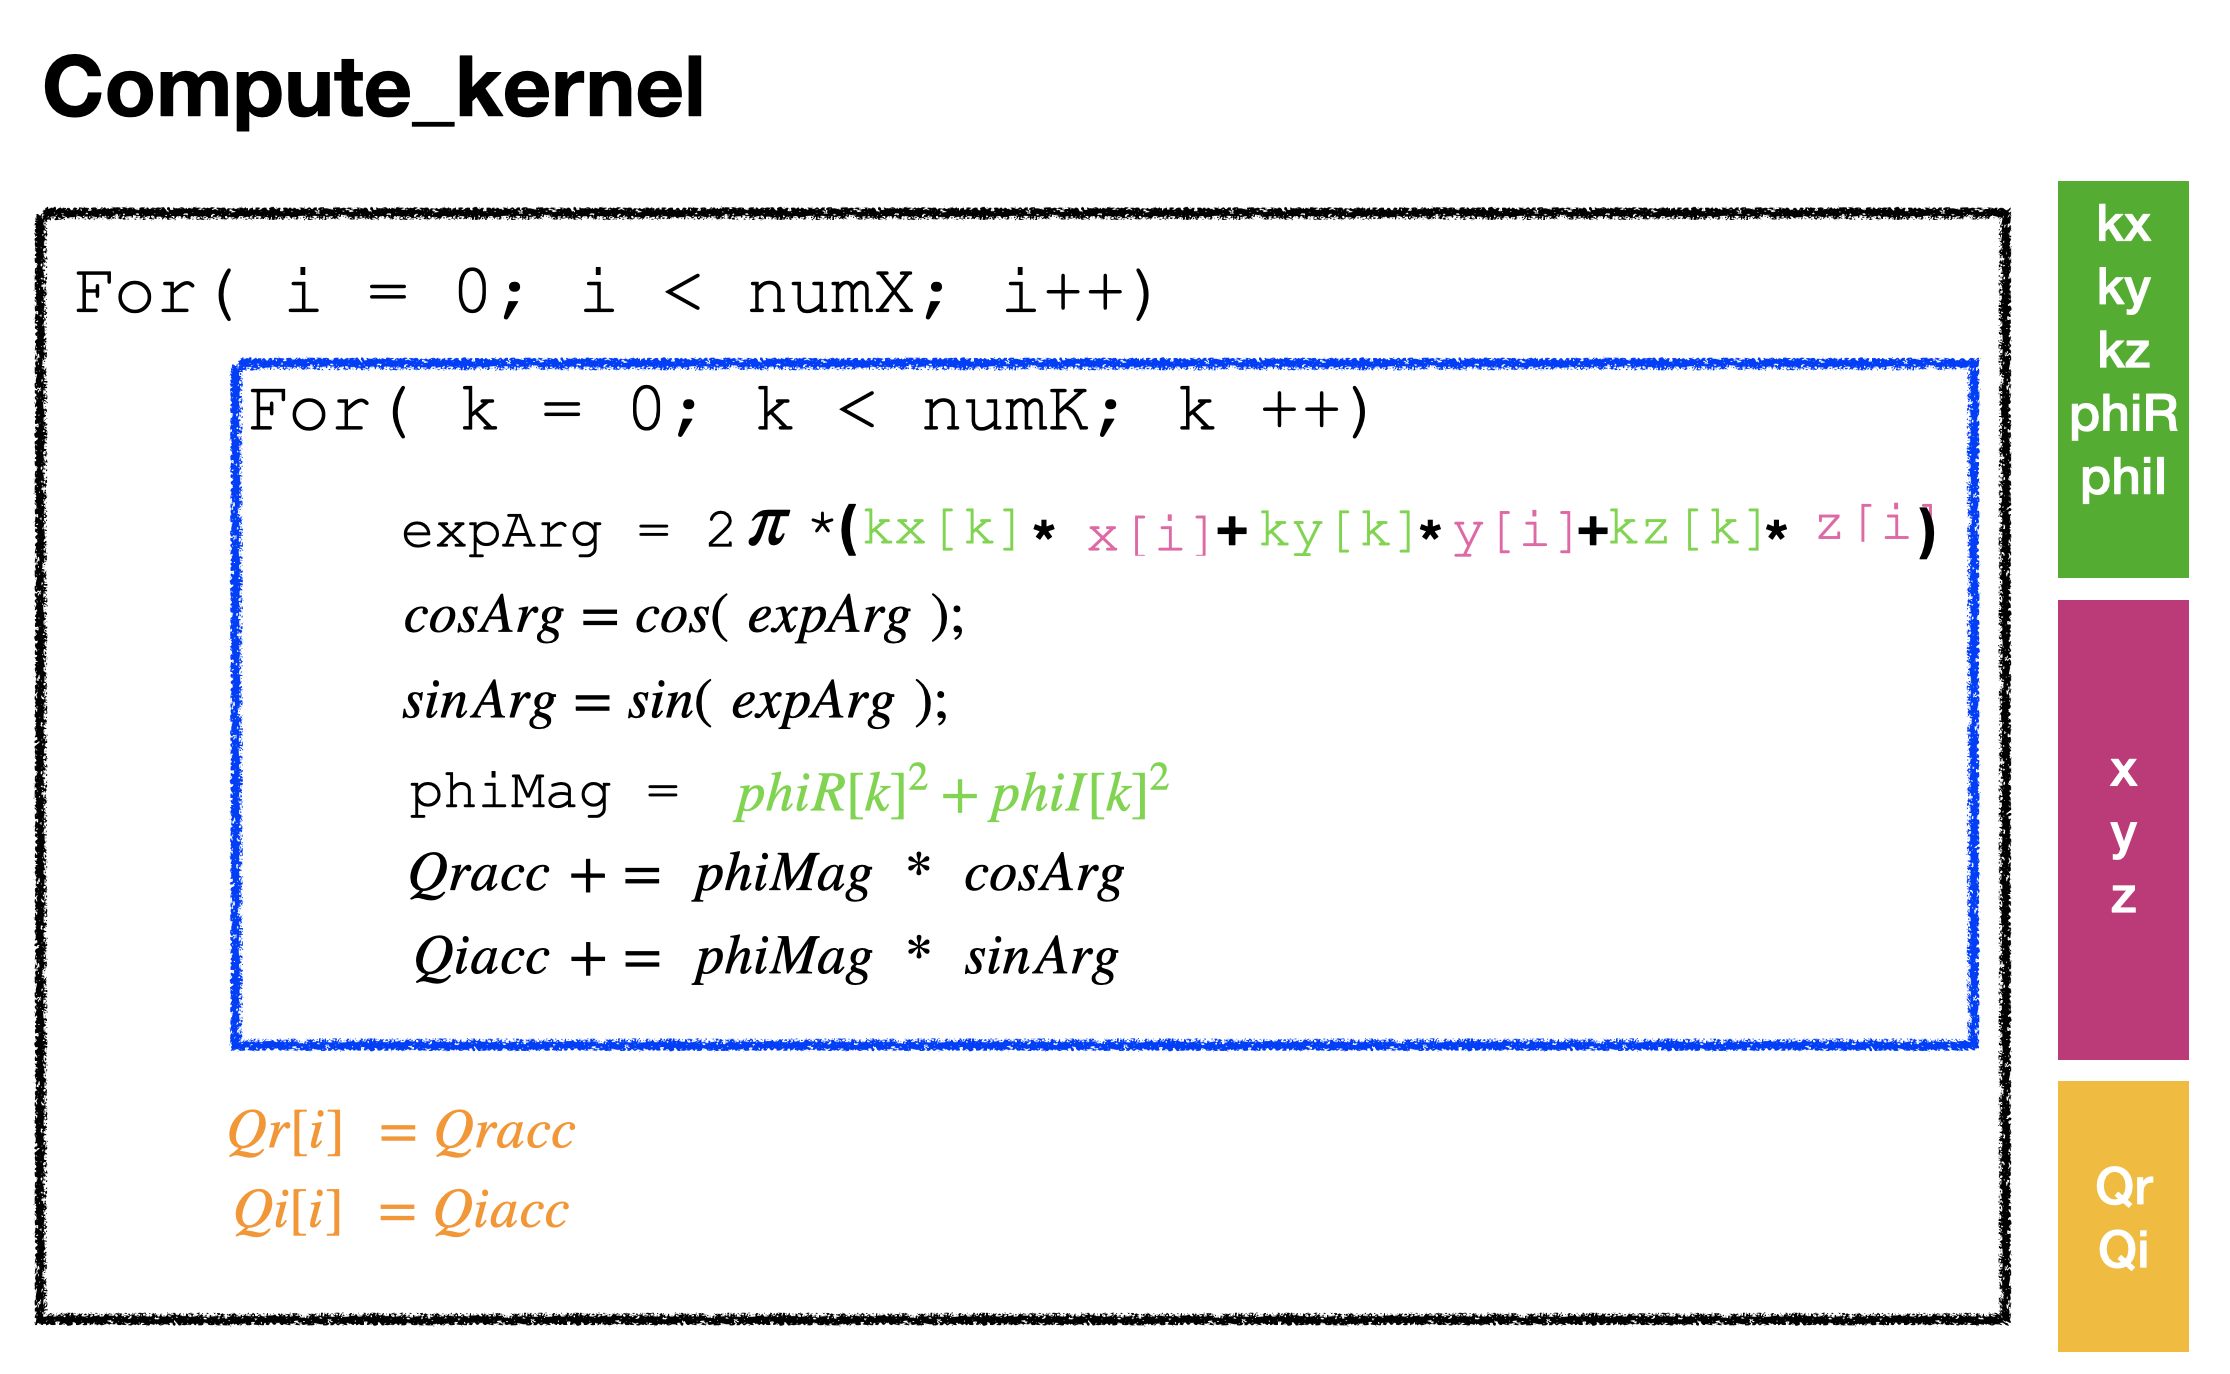
\includegraphics[width=0.85\columnwidth]{figure/algorithm.png}
\caption{Algorithm for computing MRI Q matrix~\cite{stone2008accelerating}}
\label{fig-1}
\end{figure}



\section{Progress}

\subsection{Programmer View Implementation}
\subsubsection{Implementation From the Benchmark}
The Parboil benchmark provides datasets to run the programmer view implementation. In their github repository~\cite{Rub1}, we can find documentation of this benchmark. After cloning the whole Parboil to local, under the Parboil folder, I ran the benchmark by the following command:
$$\text{./parboil run mri-q cpu small}$$
Here, ``small“ means the dataset is stored under ``small" folder, whose input image size is 32*32*32. I have also ran the test for ``large", whose input image size is 64*64*64. The image size of the largest dataset is 128*128*128.  The bigger the input data size, the higher precision of the reconstructed image.The running time for small and large are around 4.7s and 18.7s, respectively. But for the ``128x128x128" input dataset, the run time is 186685s$ \sim$ 2.2 days. This implementation was done on the socp03.cs.columbia.edu google cloud server with two cores.
\begin{table}[]
    \centering
    \begin{tabular}{c|c|c|c}
    \hline
    \hline
       name  & image size & \# of pixels & K-space dimension  \\
        \hline
    \hline
        small  & 32*32*32 & 32768 & 3072 \\
        large & 64*64*64 & 262144 & 2048\\
        128*128*128 & 128*128*128 & 2097152 & 2097152\\
        \hline
        \hline
    \end{tabular}
    \caption{Datasets of MRIQ from Parboil Benchmark}
    \label{tab-1}
\end{table}
\subsubsection{Implementation From Modified C Code}
In order to have a comparison between hardware implementation and software implementation, we need to run the software version on the processor of our SoC on FPGA. So I modified the software C code and put this implementation as a function call in the sw/linux/app/mriq.c code.\\

\subsection{Design MRIQ Accelerator in SystemC}

The MRIQ application is to compute the Q matrix. Each element of the Q matrix is a complex number with imaginary and real part. The input data can be divided into two groups. One group is coordinates information from frequency space, which is called k-space data. The other group is the sampling positions in 3-D space, which is sometimes called sampling space data. There are 5 variables from k-space, and 3 variables from the sampling space. Each pair of output is computed by using one sampling space point accumulating through the whole k-space. For the ``small" and ``medium" dataset in Table \ref{tab-1}, it has 15 K words at most for k-space data. The storage requirement is 60 K Bytes if data width is 32-bit. The whole k-space data can be stored into PLM. While for the ``large" dataset, it is 20 M words, which is 80 M Bytes. For some potential unknown applications with even higher image resolution, the storage requirement for k-space data could be larger. The storage cost may be so high that we want to sacrifice speed. For a specific application, the designer should balance the storage cost and speed requirements. For the MRI-Q matrix application, the Q matrix computation is not in real-time, so we may want to save the cost of storage and compromise on speed. Thus we need at least two architectures to deal with different input image sizes. One is called A0 dealing with small k-space data, the other is A1 dealing with large k-space data.\\



\subsubsection{Configuration Parameters}

There are two parameters provided by the benchmark, numX and numK. Since we might deal with one batch data one time, we set four parameters in total: batch\_size\_x, batch\_size\_k, num\_batch\_x, and num\_batch\_k. And they have the following relationships with numX and numK:
    $$numX = batch\_size\_x * num\_batch\_x$$
    $$numK = batch\_size\_k * num\_batch\_k$$
$batch\_size\_x$ denotes the size of one batch for sampling space data. $num\_batch\_x$ indicates how many batches needed to load the whole sampling space data. These four configuration parameters are suitable for both A0 and A1 architecture. While for A0 architecture, $num\_batch\_k$ is always 1, and $batch\_size\_k$ should be equal to $numK$.\\

\subsubsection{PLM Design}
The private local memories of accelerator is generated by "memgen" script provided by ESP. We need a script to tell memgen what kind of PLMs we need. There are three aspects we need to consider when designing PLM for MRI-Q accelerator. Firstly, the word size of the PLM. Input variables from sampling space and output have the same size, while PLMs storing k-space data should have a different word size. Additionally, PLMs storing k-space variables customized for A0 architecture should have size of $numK$, while it should be $batch\_size\_k$ for A1. Secondly, DMA width of the processor core. In order to maximize the latency performance, we can customize ports of PLMs to work with different processor cores. For example, Ariane core has 64-bit DMA width, the PLM should provide two writing ports when loading data into PLM in parallel. while one port is enough for Leon3 core with 32-bit DMA width. Thirdly, parallelism level. In compute phase, how many data we can access in parallel is determined by number of the corresponding PLM ports. For example, if we wanted to do 4 computation in parallel, the PLM which stores the input data should have 4 reading ports. Then we should specify in the hw/mriq\_directives.hpp file that what memory we want to use under what conditions. 


\subsubsection{Data Type}

Since the FPGA can not process floating-point data directly, we need to do various data conversions in both the accelerator and the testbench. fpdata.hpp file defines functions used to do datatype conversions, including int2fp(), fp2int(), fp2bv(), bv2fp(). The data conversion flow is concluded in Fig.\ref{fig-data-convert}. In the testbench, data in floating-point type read from files is converted to fixed-point representation, then converted to sc\_bv to be transported through the network-on-chip. In accelerator, data in sc\_bv  type is converted to sc\_int to be stored in PLM. In computation phase, sc\_int data is converted back to fixed-point representation. After computation finished, The fixed-point data needs to be converted back to sc\_int to be stored in PLM. Then, it is further converted to sc\_bv to be transported back to the testbench for validation. In testbench, sc\_bv is converted to fixed-point representation. and further converted to floating-point type to be compared with the golden output data. \\
\begin{figure}[t]
\centering
\captionsetup{justification=centering, format=hang}
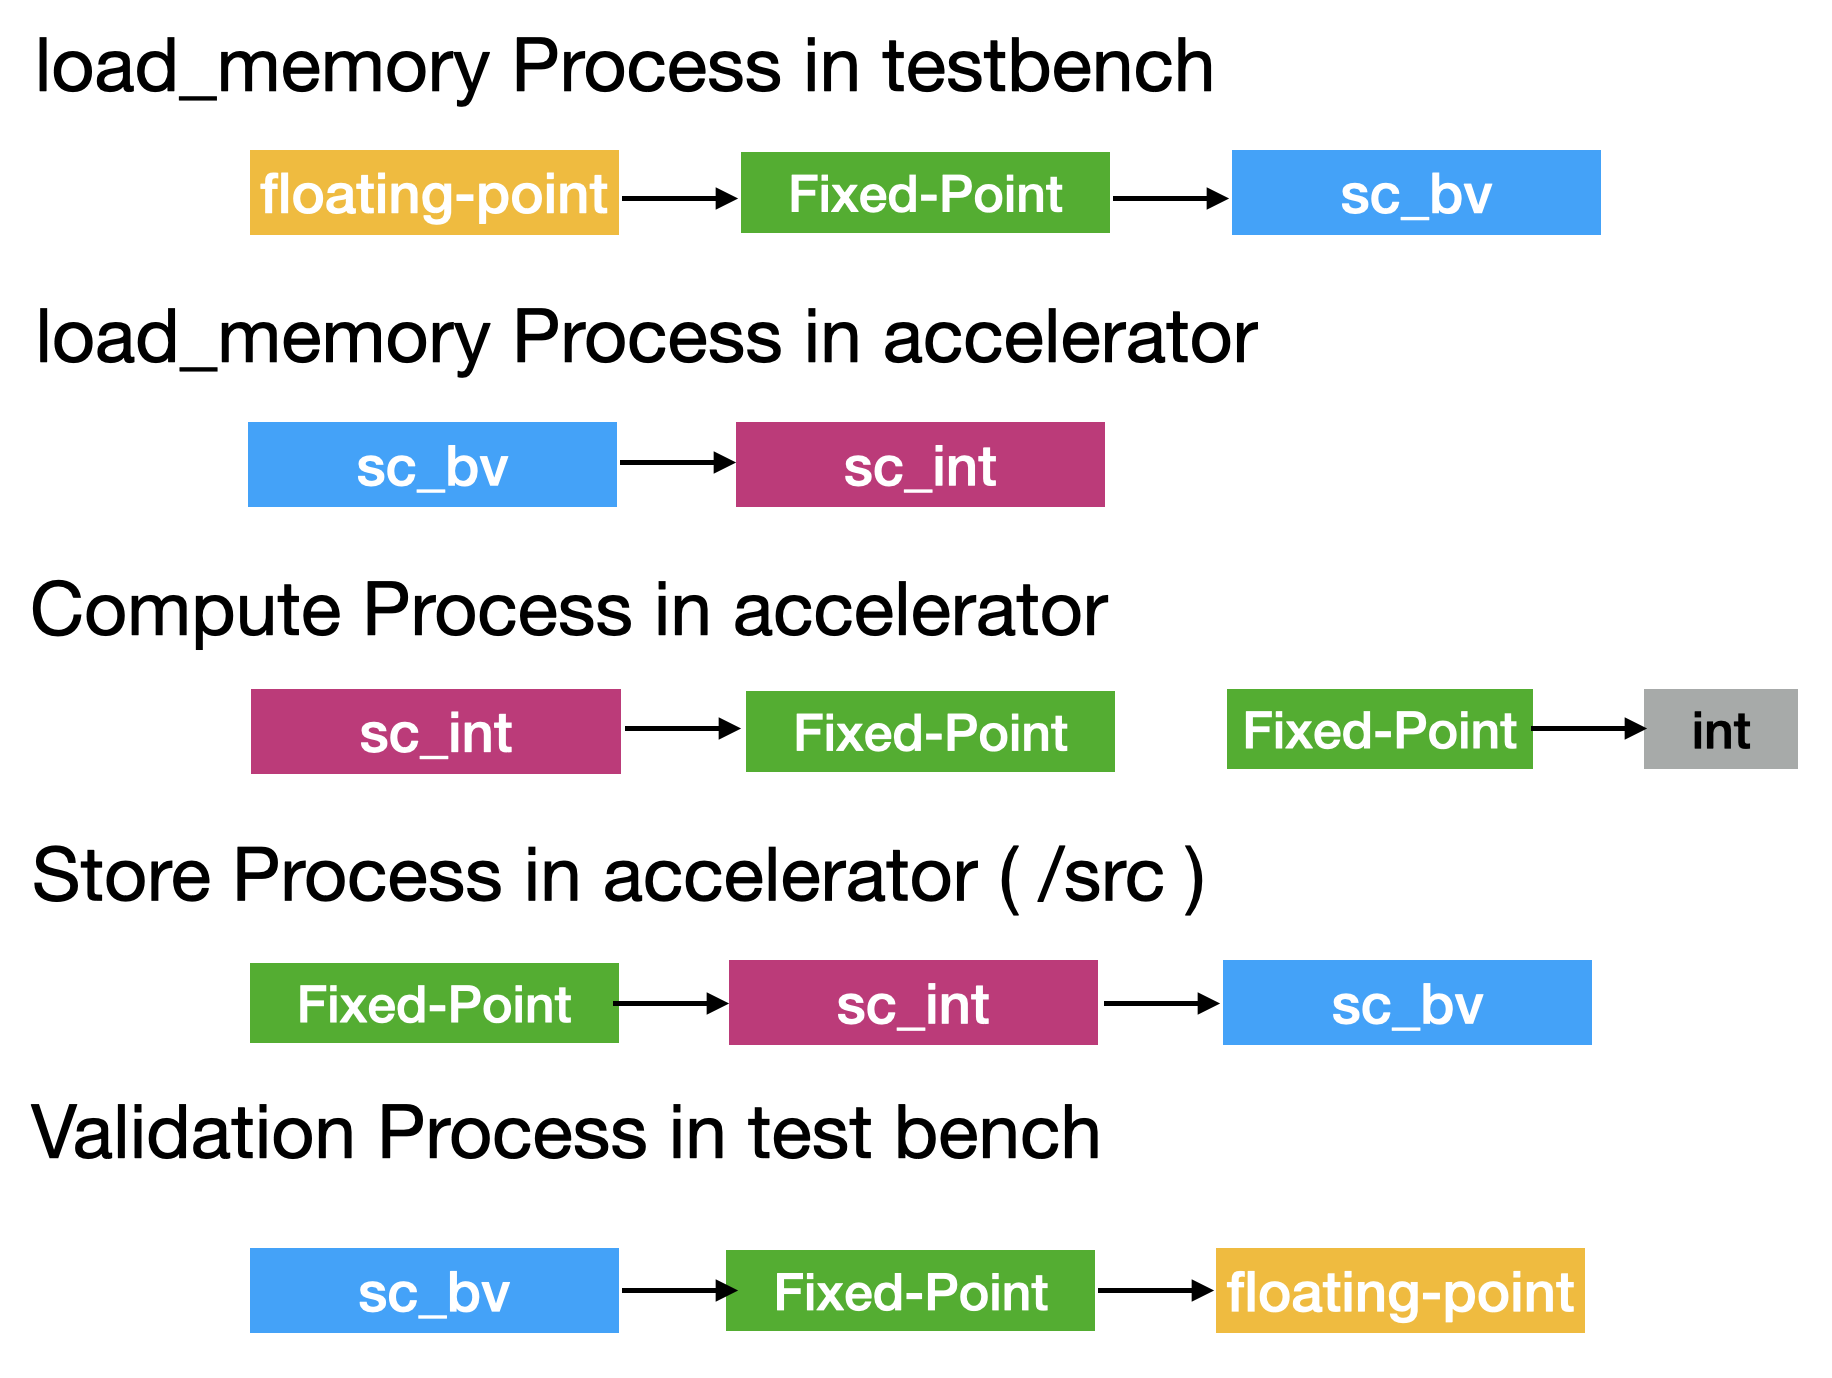
\includegraphics[width=0.85\columnwidth]{figure/data-conversion.png}
\caption{Data conversion in testbench and accelerator}
\label{fig-data-convert}
\end{figure}



\subsubsection{Functions}
There are four functions essential to MRI-Q accelerator design. In load process, \textit{load\_data()} function is to load data into different PLMs. This function loads "len" number of words, starting with dma address "dma\_addr", into a PLM with name "array". In this function, dma\_info is configured first, including dma\_addr, dma\_length, and dma\_size. Then it stores data from dma\_read\_chnl to PLM "array".
$$\mathrm{load\_data(array[], dma\_addr, len)}$$
 The second function is \textit{store\_data}, which is the counterpart of load\_data(). It sends data stored in "array" PLM through dma\_write\_chnl to the testbench.
$$\mathrm{store\_data(array[], dma\_addr, len)}$$
The third function is \textit{computeQ} which is to compute a pair of output data with the whole k-space variables and one sampling space data point (x, y, z). In computeQ, there are three tasks being pipelined. The first task is reading data from PLM into registers kx, ky, kz, phiR, and phiI. The second task is to do the computation part. The third taks is to accumulate the intermediate results. After the loop finishes, it stores the accumulated results into two memory addresses pointed by pointers Qr and Qi.
$$\mathrm{computeQ(x, y, z, batch\_size\_k, pingpong\_x, sin\_table, *Qr, *Qi)}$$

\begin{figure}[t]
\centering
\captionsetup{justification=centering, format=hang}
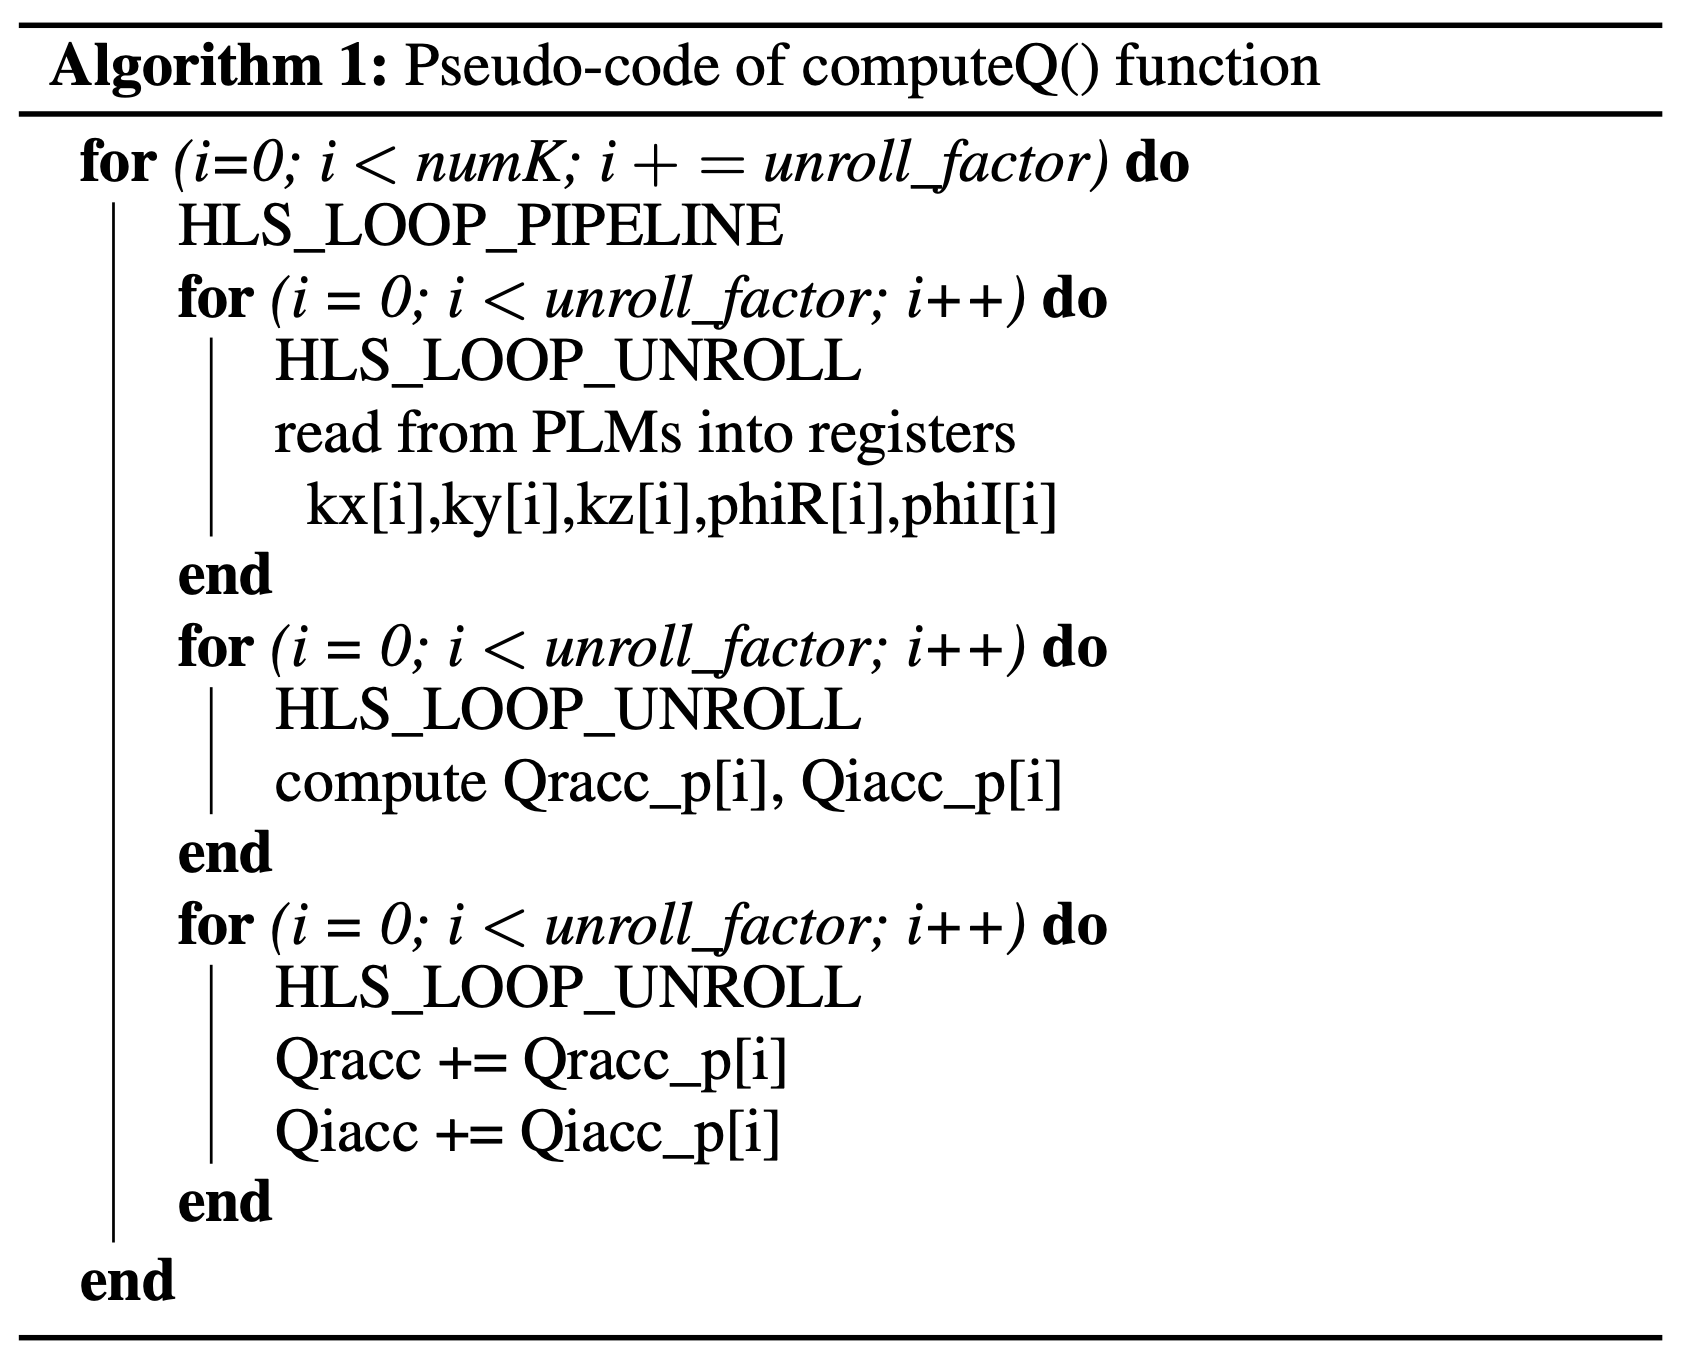
\includegraphics[width=\columnwidth]{figure/computeQAlgorithm.png}
\label{fig-data-convert}
\end{figure}



The fourth function is \textit{mySine} which is to compute the sine value of an input.
$$\mathrm{mySinf(angle, sin\_table)}$$
The algorithm in Fig.\ref{fig-1} shows that it needs to compute triangular functions, sine and cosine. Since Stratus HLS doesn't provide sine and cosine function, we implemented a sine function \textit{mySine}. We firstly convert any input value to $0~\pi/2$ range, $x$, then find the closest data point to $x$ in the sin\_table, then do interpolation to get sin(x). 
\\

\subsubsection{Processes}
In the main hardware design source file mriq.cpp, we have three processes, load\_input, compute\_kernel, and store\_output. load\_input handshakes with compute\_kernel. compute\_kernel handshakes with store\_output. These three processes are pipelined in the background. For both A0 and A1 architectures, we are utilizing ping-pong buffers to store sampling space variables (x, y, z) and (Qr, Qi). A flag pingpong\_x is to tell each processes whether we should read from or write to plm\_var\_ping or plm\_var\_pong memory. For A1 architecture, we also need ping-pong buffers to store k-space variables. Thus we need another flag pingpong\_k as a local variable in each process. Conditional loading in the load\_input process is implemented. We have a counter variable counting how many times load\_input process has been implemented. Whenever we load one batch of sampling space variables, we need to load k-space variables for $num\_batch\_k * batch\_size\_x$ times, and we flip pingpong\_k flag and handshake with compute\_kernel process for every loading. Then we flip pingpong\_x and reset the counter in load\_input process. After the computation of the current batch of sampling space variables finishes, we flip pingpong\_x flag once and handshake with store\_output process in compute\_kernel process. \\

\subsection{Testbench Design}
 The ESP provides skeleton code for the testbench design. We only need to fill in customized code in each function. In tb/system.hpp file, it defines a class system\_t. In this class declaration, there is a constructor function, and other members. For example, configuration parameters to the accelerator, variables used by different methods, and methods. Here we declare an additional method used by load\_memory function, which is load\_mem() method. In system.cpp file, we have four methods definitions. In load\_memory(), we initialize the necessary parameters first, then fill the "mem" variable with input data and fill the "gold" pointer with golden output data. Since the accelerator can only deal with fixed-point data, we convert floating-poing data to sc\_bv to be transported to the accelerator. In dump\_memory(), we convert and store the output sent from the accelerator to a pointer variable "out" with floating-point type. In validate(), we compare "out" with "gold" to verify the accelerator design. \\
 \\
 We define some helper functions in a separate folder, "common" folder. In the testbench design, we used init\_parameter() and validate\_buffer(), defined in utils.h file. These two helper functions are also used in software testing application code.\\

\subsection{Software Testing Applications}

ESP enables two testing on FGPA. One is bare metal application testing and the other is testing the accelerator with Linux OS. These two applications are in sw/ folder. \\
\\
For the bare metal application, we need to fill in code in init\_parameters(), init\_buf() and validate\_buf(). Since bare metal implementation doesn't support many C librabries, we can't use init\_buffer function in common/utils.h file. We generated testing input data beforehand and included it as a file. While in validate\_buf function, we first convert output sent from the accelerator from fixed-point data to floating-point data by using fixed32\_to\_float() function provided by fixed\_point.h. Then use validate\_buffer() function from common/utils.h to validate the output. \\
\\
For linux application, we also only need to fill customized code in init\_parameters(), init\_buf(), and validate\_buf() function, same as the bare-metal application except the init\_buf() function. Since we run the test program on linux OS,  the init\_buf can use the function init\_buffer() in common/utils.h, which reads input data from file. We can also test the execution time of software program running on the processor tile of SoC which is prototyped on the FPGA. When running the linux application, we pass three arguments: name of input File, name of output file, and the answer to whether we want to run software program with "0" indicating "no" and "1" indicating "yes". 
\\
\subsection{Testing Results}

The testbench can help us debugging our accelerator at design phase. When we don't have "\#if" directives, we can run behavioral simulation by running make target "make mriq\_stratus-exe". This will check if our accelerator has the expected behavior. Then we can generate RTL with "make mriq\_stratus-hls" and simulate RTL with the testbench. When we use "\#if" directive to generate multiple RTL implementations, the above three make targets won't work correclty. Then we need to use the debugging method provided on the ESP tutorial, which is to simulate one specific RTL with "make debug\_<RTL name>". For example, if we want to test A1 architecture with DMA width as 64 and parallelism level as 4, we can run "make debug\_BASIC\_P4\_A1\_DMA64\_V". The running result is shown in Fig.\ref{fig-3}. 
\\
\begin{figure}[ht]
\centering
\captionsetup{justification=centering, format=hang}
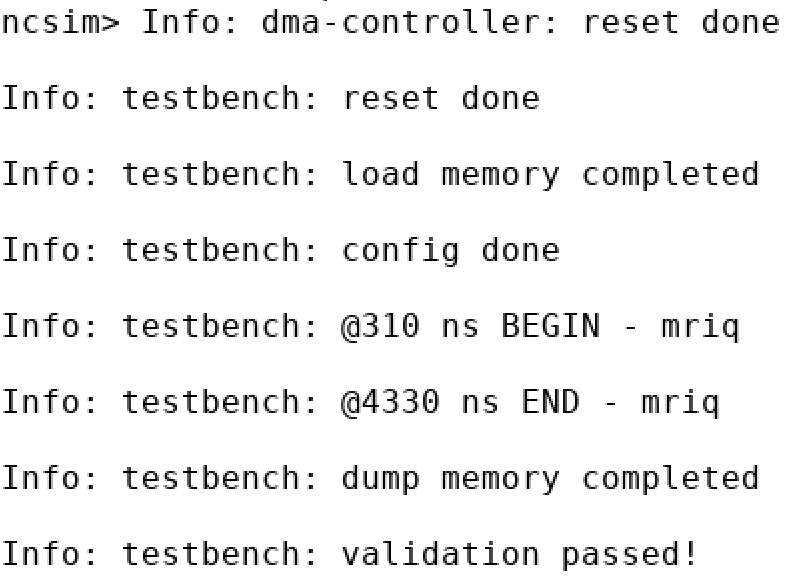
\includegraphics[width=0.75\columnwidth]{figure/reverted-debug-sim-A1-4-4-2-2.png}
\caption{RTL simulation (BASIC\_P4\_A1\_DMA64\_V)}
\label{fig-3}
\end{figure}
\\
After we finish the software testing program design, we can also simulate and test the bare metal application, and run the Linux application after booting the FPGA with Linux image. For the baremetal application, for example, we test "P4\_A0\_DMA64" RTL on FPGA, the result is shown in Fig.\ref{fig-barec-app}. If we generated Linux image and registered the mriq\_stratus accelerator as a device driver, we can test the linux app on FGPA. The running result is shown in Fig.\ref{fig-linux-app}. Fig.\ref{fig-linux-app}-(a) shows that we also ran the software program on the SoC core, and the execution time is roughly 10 times slower than the hardware accelerator on a small testing data.

\begin{figure}[t]
\centering
\captionsetup{justification=centering, format=hang}
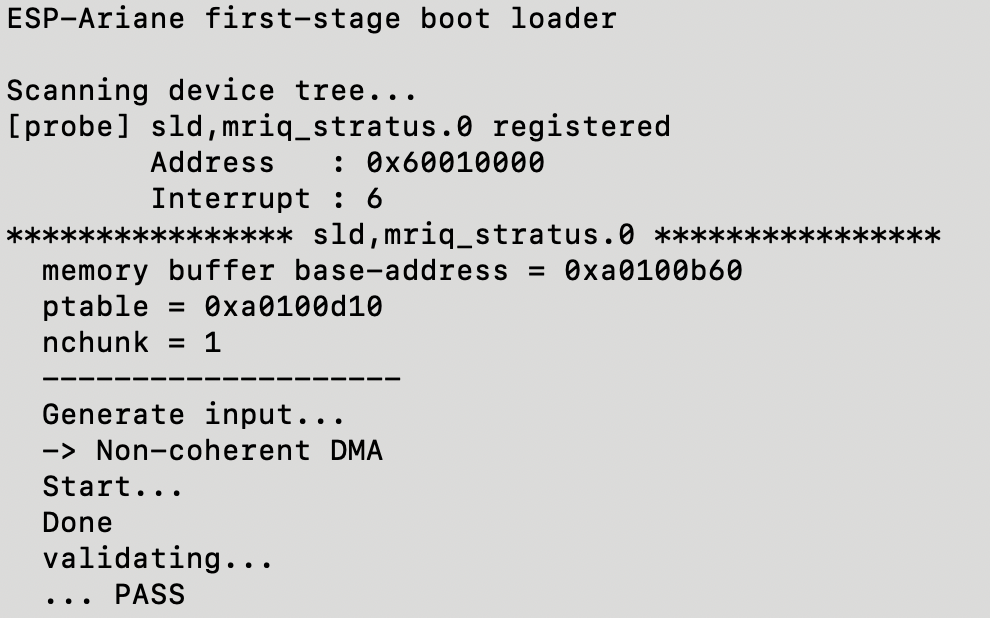
\includegraphics[width=0.85\columnwidth]{figure/reverted-barec.png}
\caption{Running bare metal app on FPGA}
\label{fig-barec-app}
\end{figure}

\begin{figure}[t]
\centering
\begin{subfigure}{.5\columnwidth}
\centering
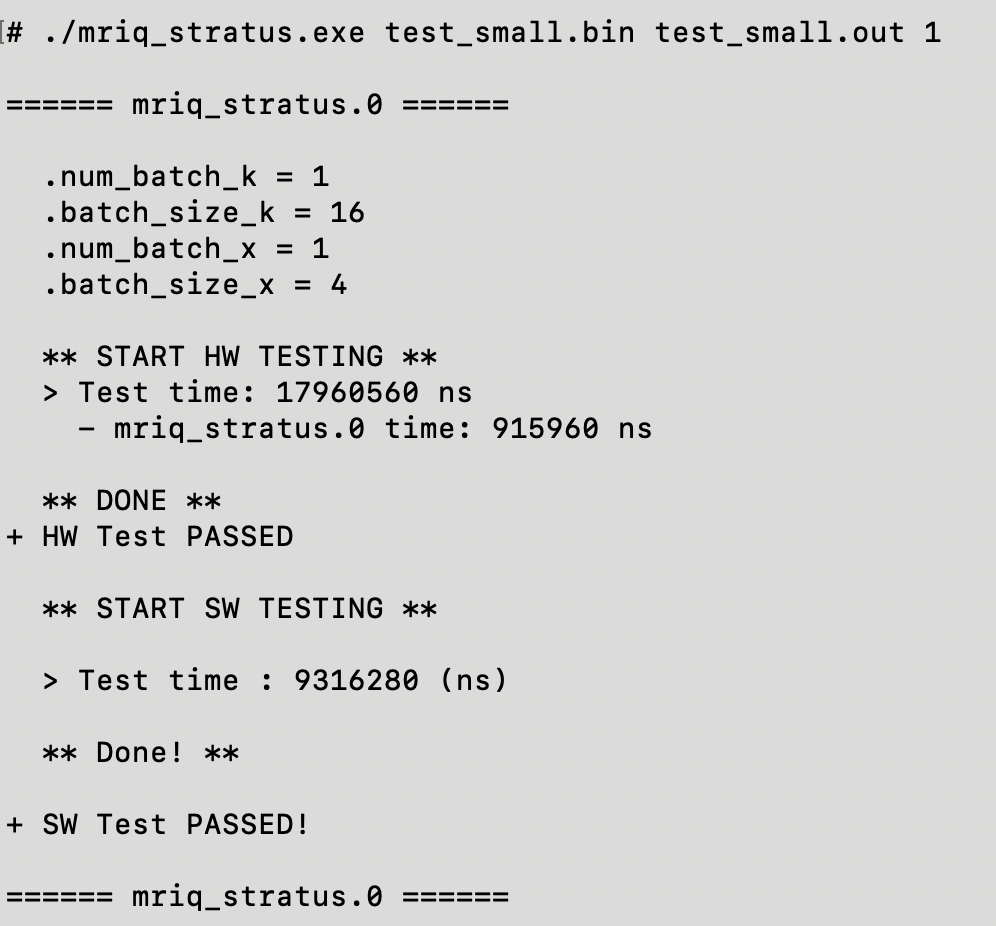
\includegraphics[width=\columnwidth]{figure/reverted-color-linux-run-sw.png}
\caption{w/ running sw}
\end{subfigure}%
\begin{subfigure}{.5\columnwidth}
\centering
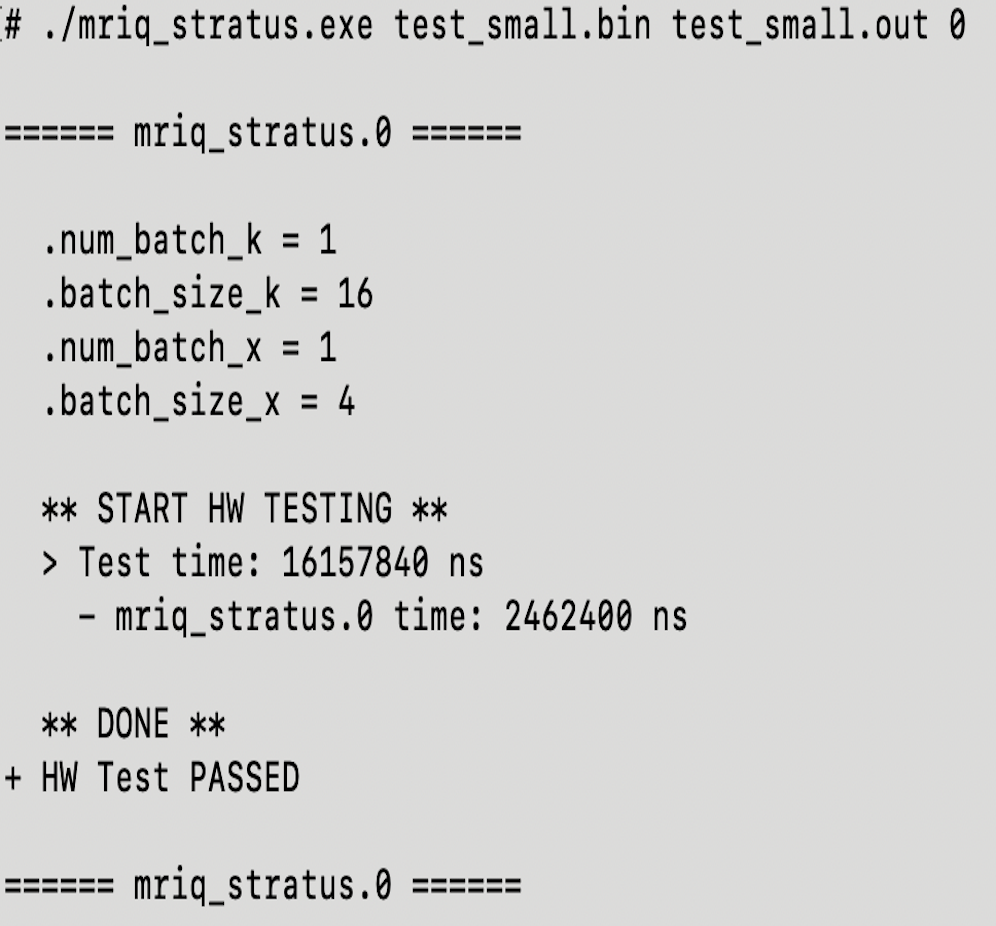
\includegraphics[width=\columnwidth]{figure/inverted-linux-app-wo-run-sw.png}
\caption{w/o running sw}
\end{subfigure}
\caption{Running Linux app on FPGA}
\label{fig-linux-app}
\end{figure}


\section{Design Space Exploration}
After we fixed the basic architectures of the design. We can try different HLS knobs to optimize our accelerator from area and latency directions. \\
\subsection{Low Area Optimization}

\subsubsection{Customize PLM}
We want to customize PLM size for two different input variables. k-space variables have the same size while sampling-space variables have the same size but different from the k-space variables. So we set different PLMs for these two groups. \\
\\
Since we can customize number of ports for each PLM, we shouldn't waste any ports in order to save area. For PLMs storing input data, we set the number of writing ports accordingly to be consistent with DMA width. For example, if DMA width is 64, while data width is 32, then there are two writing ports. If DMA width and data width are both 32, then we only need one writing ports. The number of reading ports of different PLMs depends on the parallelism level. If parallelism level is 4, we need to read 4 k-variables in parallel in the compute\_kernel process. So 4 reading ports are needed.\\

\subsubsection{Fixed-Point Datatype Optimization}
The MRI-Q accelerator deals with fixed point datatype. We can reduce fixed point precision to reduce both latency and area. When we have only one type of fixed-point data representation and reduce the word length to 29, there are no errors in output data and both area and latency reduced. Further reduction in word length led to output errors. In order to further reduce the data width of the fixed-point representation, I analyzed all the testing data provided by the Parboil benchmark suite. Some data are bound to be very small value, for example, the output of trigonometric functions is always less than 1, and some are large values. The range of data are shown in Table.\ref{tab-8}. I set two different fixed-point representations, shown in Table.\ref{tab-4}. We use FPDATA\_S to represent kx, ky, kz, phiR, phiI, x, y, z, and phiMag, sinArg, cosArg. And we use FPDATA\_L to represent the other variables. The result shows that the error rate is 0.17\% when error threshold (percentage difference between computed output and golden output), is set as 5\%. So the data width can be as small as 24 compared to 32. \\
\begin{table}[h!]
    \centering
    \begin{tabular}{c|c|c|c}
    \hline
        & WL & IL & Fractional Bits \\
        \hline
   FPDATA\_S &  24  & 5  & 19 \\ 
FPDATA\_L &  24 & 11   & 13\\
    \hline
    \end{tabular}
    \caption{Fixed-point data representation}
    \label{tab-4}
\end{table}

\begin{table}[ht!]
    \centering
    \begin{tabular}{c|c|c|c}
    \hline \hline
   Variables &       Max&    Min& Integer bits\\
   \hline \hline
 x&     3.083235        &-0.500000& 3 \\
 y&     0.484375        &-0.500000& 1 \\
 z&     0.484375        &-0.500000& 1 \\
 kx&    10.889303       &-10.889303& 5 \\
 ky&    16.019472       &-16.019472& 5 \\
 kz&    0.585179        &-0.585179& 1\\
 phiI   &0.484375       &0.312500& 0 \\
 phiR   &0.484375       &0.406250& 0 \\
 phiMag &0.469238       &0.262695& 0 \\
 cosArg&        1.000000        &-1.000000& 2\\
 sinArg &1.000000       &-1.000000& 2 \\
 \hline
 expArg &226.168869     &-226.168869& 9 \\
 Qracc  &961.000000     &-472.693146& 11 \\
 Qiacc  &97.710320      &-97.710320& 8 \\
\hline \hline
    \end{tabular}
    \caption{Value range for all variables}
    \label{tab-8}
\end{table}




We experimented with small data set and we extracted area from the synthesized RTL and extracted latency data from RTL simulation. This small dataset has numX as 4 and numK as 16, and it is running with accelerator A0\_P4\_DMA64. The extracted area and latency data are shown in Table.\ref{tab-3}. Area reduces by 31.5\%. Latency also reduces by 11.49\%. But when we simulate the bare-metal application, it doesn't support data width as 24. So we set FPDATA\_S and FPDATA\_L with the same specification (WL, IL) = (32, 12) in the other evaluations.
\\
\begin{table}[h!]
    \centering
    \begin{tabular}{c|c|c|c}
    \hline
        & $WL=32$ & $WL=24$ &  Gain \\
        \hline
   area &  0.1185  & 0.0812   & -31.50\% \\ 
latency (ns) &  1740 &  1540  & -11.49\% \\
    \hline
    \end{tabular}
    \caption{Performance of FP precision reduction}
    \label{tab-3}
\end{table}
 \\ 




\subsection{Low Latency Optimization}
We have two directions to reduce latency. The first one is to accelerate the loading and storing process. The second one is to accelerate the computation. Since the data transportation between processor and the accelerator is done in serial, we can increase the burst rate and DMA width. In our case, burst rate is fixed and the DMA width is determined by the processor core we have in our SoC. The Ariane core provides DMA width as 64-bit, while Leon3 core has DMA width as 32-bit. In the computation phase, we can do loop unrolling and loop pipeline to accelerate. Since we don't have the choice to work on accelerating load and store process, we can only work on the compute\_kernel. \\
\\
A0 architecture loads all the k-space data into PLM. It uses ping pong buffer to load sampling space data. The RTL simulation waveform of A0\_P4\_DMA64 shows that loading one batch of sampling space data takes 2 $\mu$s with batch\_size\_x set as 128, and generating one pair of output data takes 7 $\mu$s . Thus generating 128 pairs of output data takes 900 $\mu$s. So the compute\_kernel process is dominating other processes, and the loading process of the sampling space data is totally hidden by computation process. It also means that the acceleration done on compute\_kernel will have the biggest impact on the final latency. But A1 architecture behaves very differently. When we set batch\_size\_k as 1024, loading five k-space variables takes 25 $\mu$s. If num\_batch\_k was 10, then preparing all the input to generate one pair of output takes $25\mu$s $* 10 = 250\mu$s, while the computation takes 7us to finish. Loading process is dominating for A1 architecture and any optimization to the compute\_kernel won't work. \\
\\
First, let's look at the Pareto curve of A0 architecture, which is shown in Fig.\ref{fig-paral}. The area and latency data is extracted from RTL synthesis results and RTL simulation results. The testing parameters are shown in Table \ref{tab-test-param}. The number in P-<number> indicates the unroll-factor. We can see that latency is decreasing when we increase the parallelism level. We have tried unroll factor 4, 8, 16. In the compute\_kernel process, we have three tasks which can be pipelined. The first one is to read data from PLMs to registers. The second task is to do computation, and the third task is to store the computed results. For our MRI-Q application, the third step is to accumulate the intermediate results. Every task can be unrolled for unroll-factor number of times. In order to support reading from the same PLM for unroll-factor number of data into registers in parallel , the PLM in question should have unroll-factor number of reading ports.

\begin{table}[h!]
     \centering
     \begin{tabular}{c|c|c}
        \hline
          Configurable variables& A0 & A1  \\
         \hline
         numX & 256 & 256 \\
         \hline
         batch\_size\_x & 128 & 128 \\
         \hline
         num\_batch\_x & 2 & 2 \\
          \hline
         numK & 3072 & 3072 \\  
         \hline
         batch\_size\_k & 3072 & 1024 \\
         \hline
         num\_batch\_x & 1 & 3 \\
         \hline
     \end{tabular}
     \caption{Testing Parameters of the Pareto curve}
     \label{tab-test-param}
 \end{table}

\begin{figure}[h!]
    \centering
    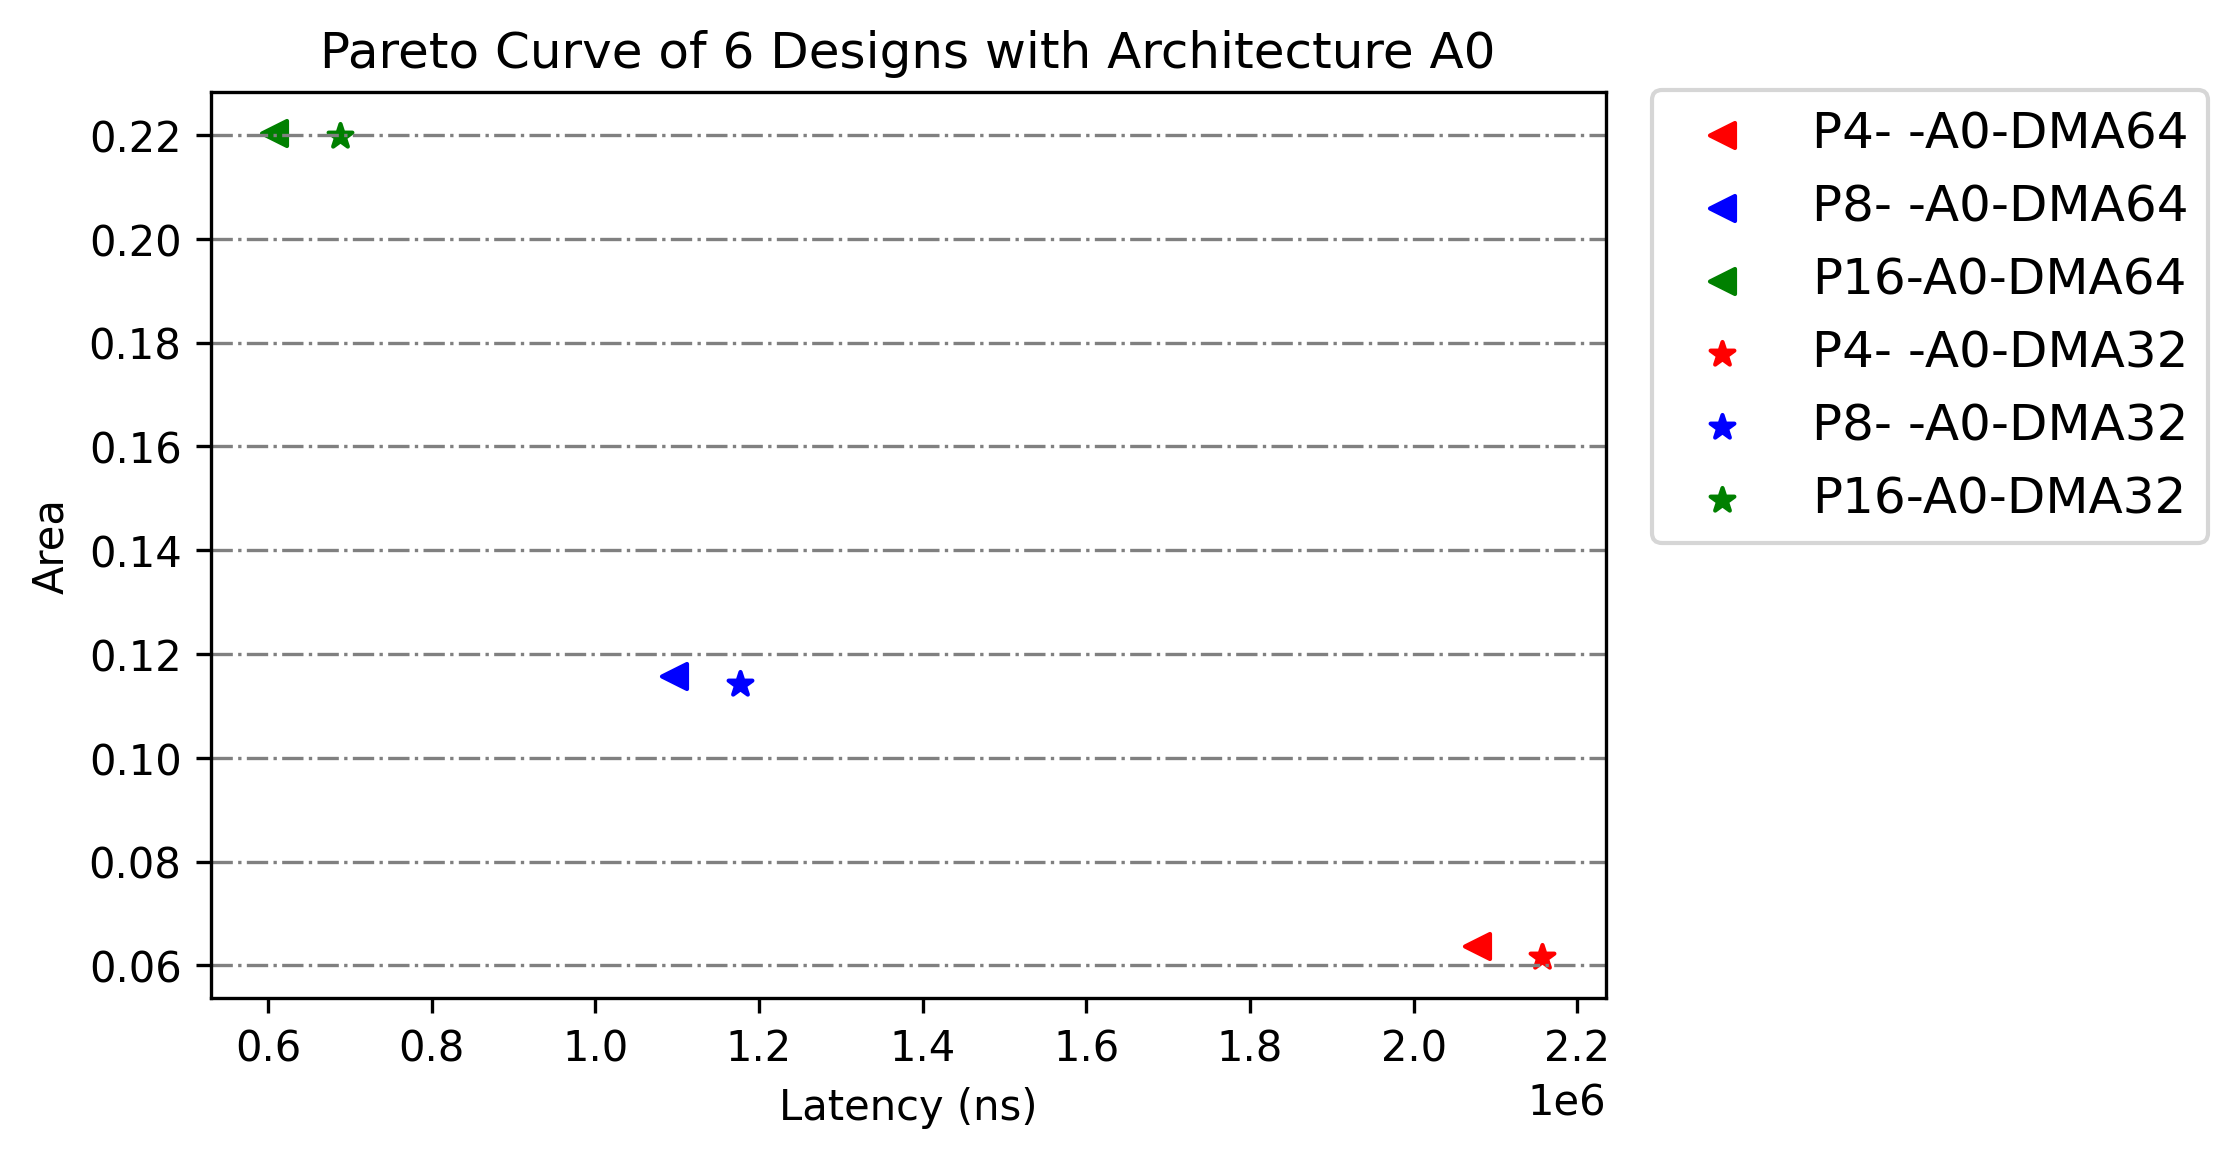
\includegraphics[width=\columnwidth]{figure/Pareto-curve-A0.png}
    \caption{Pareto curve of 6 designs of A0}
    \label{fig-paral}
\end{figure}

The latency optimization for A1 architecture should solely depend on the DMA width as we have discussed above. The optimization done in compute\_kernel shouldn't have any effect, shown in Fig.\ref{fig-a1-pareto}.\\
\begin{figure}[h!]
    \centering
    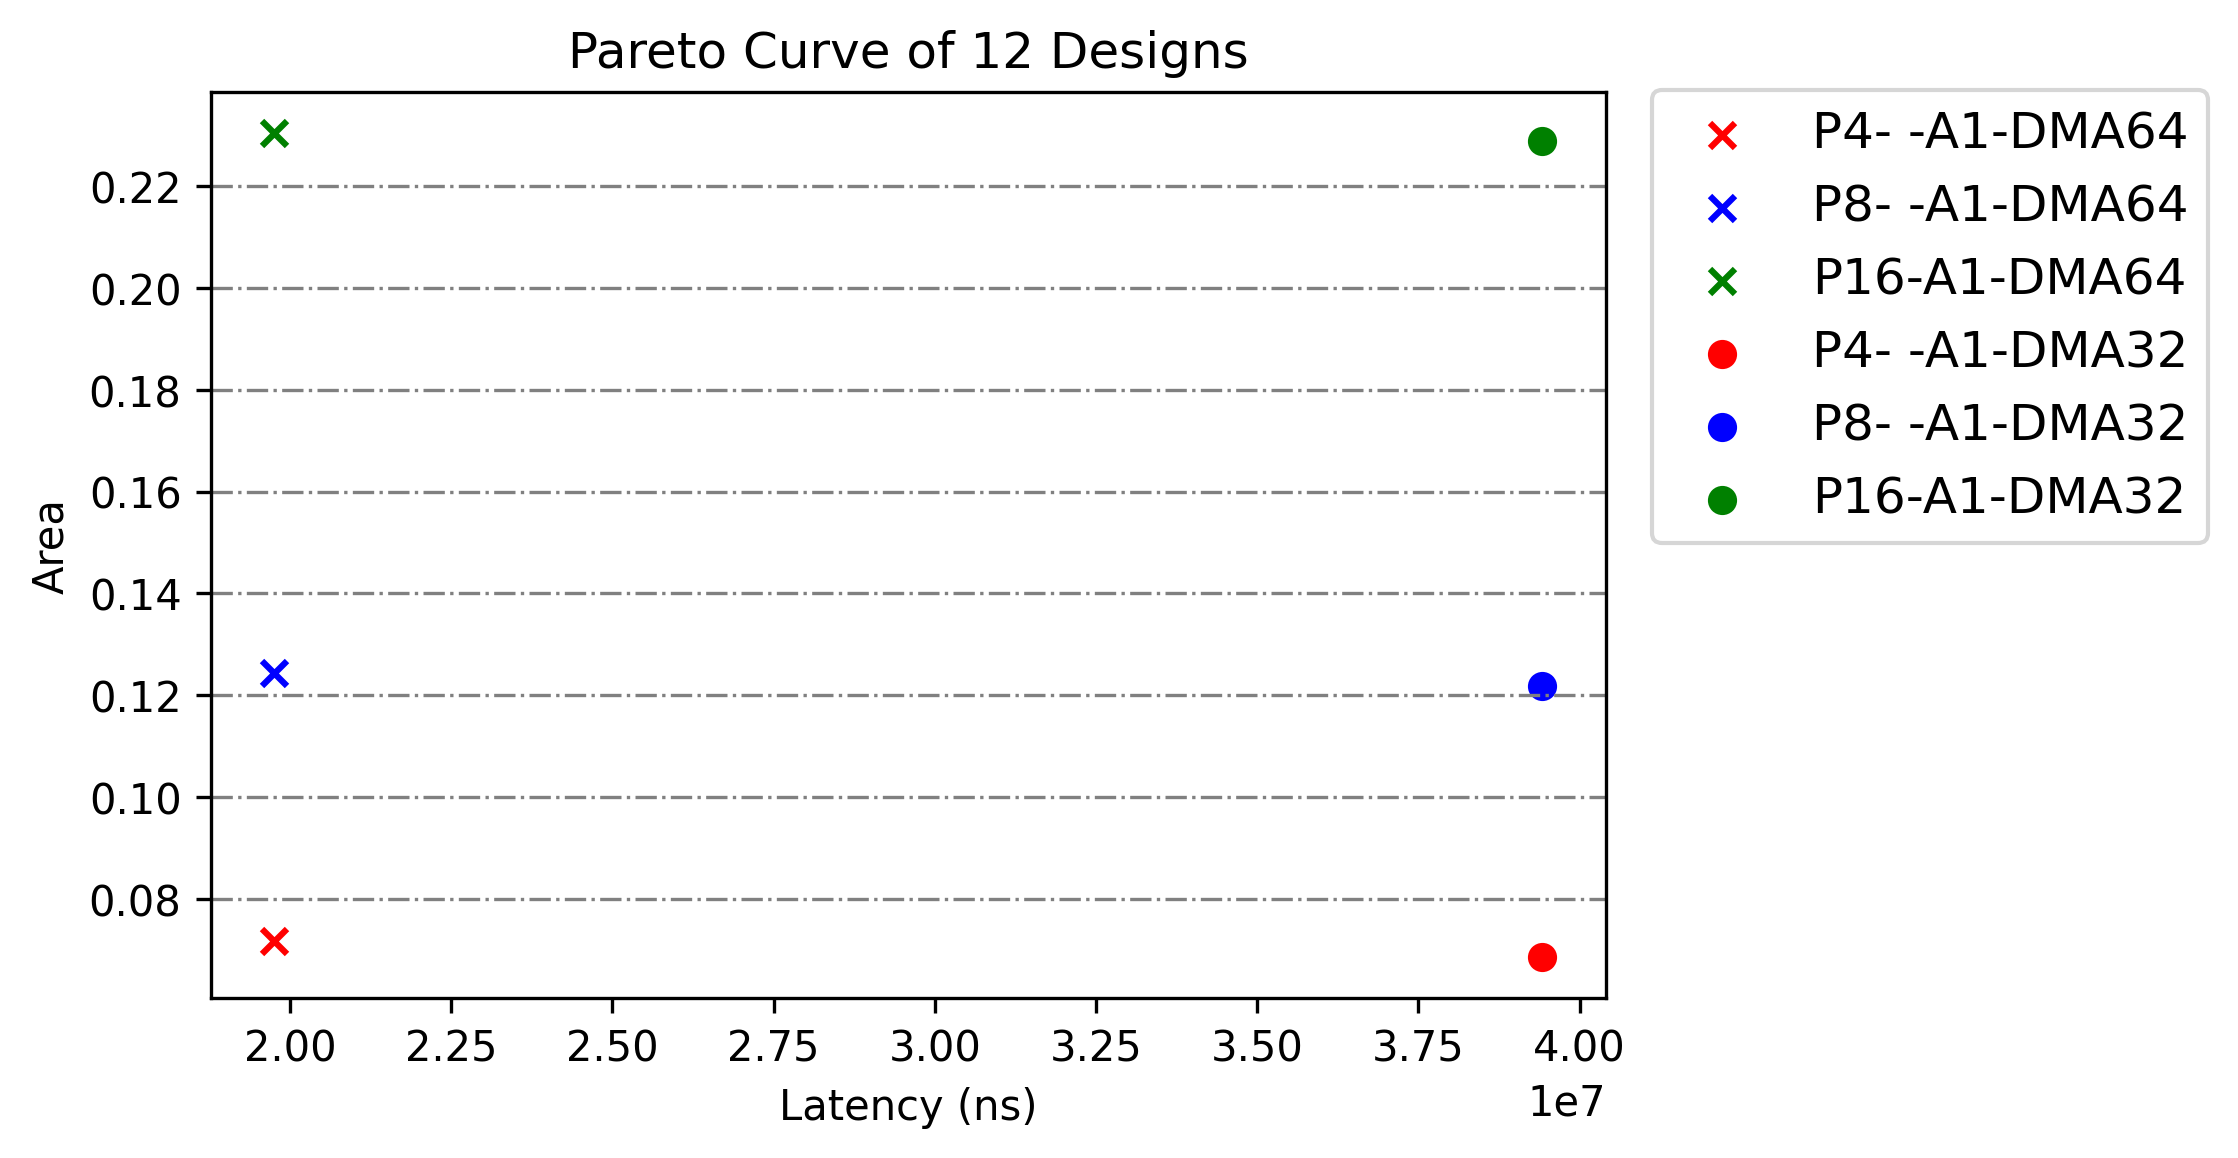
\includegraphics[width=\columnwidth]{figure/Pareto-curve-A1.png}
    \caption{Pareto curve of 6 designs of A1}
    \label{fig-a1-pareto}
\end{figure}



\subsection{Results of Testing on FPGA}

By invoking linux on FPGA, we collected both the software execution time running on the Ariane core and the execution time running on the MRI-Q accelerator. For A0 architecture, data is shown in Fig.\ref{fig-d32-64} for 32x32x32 (D32) and 64x64x64 (D64) dataset.  The right y-axis shows the speed-up of the two testing. The speed up is greater than 5000 for both datasets when parallelism level is 16. The testing result of D32 shows a slightly higher speed-up than D64 is because that numK of D32 is 1.5X of D64. Increasing parallelism in compute can improve latency, same as the extracted data from the synthesized RTL.\\

\begin{figure}[h!]
    \centering
    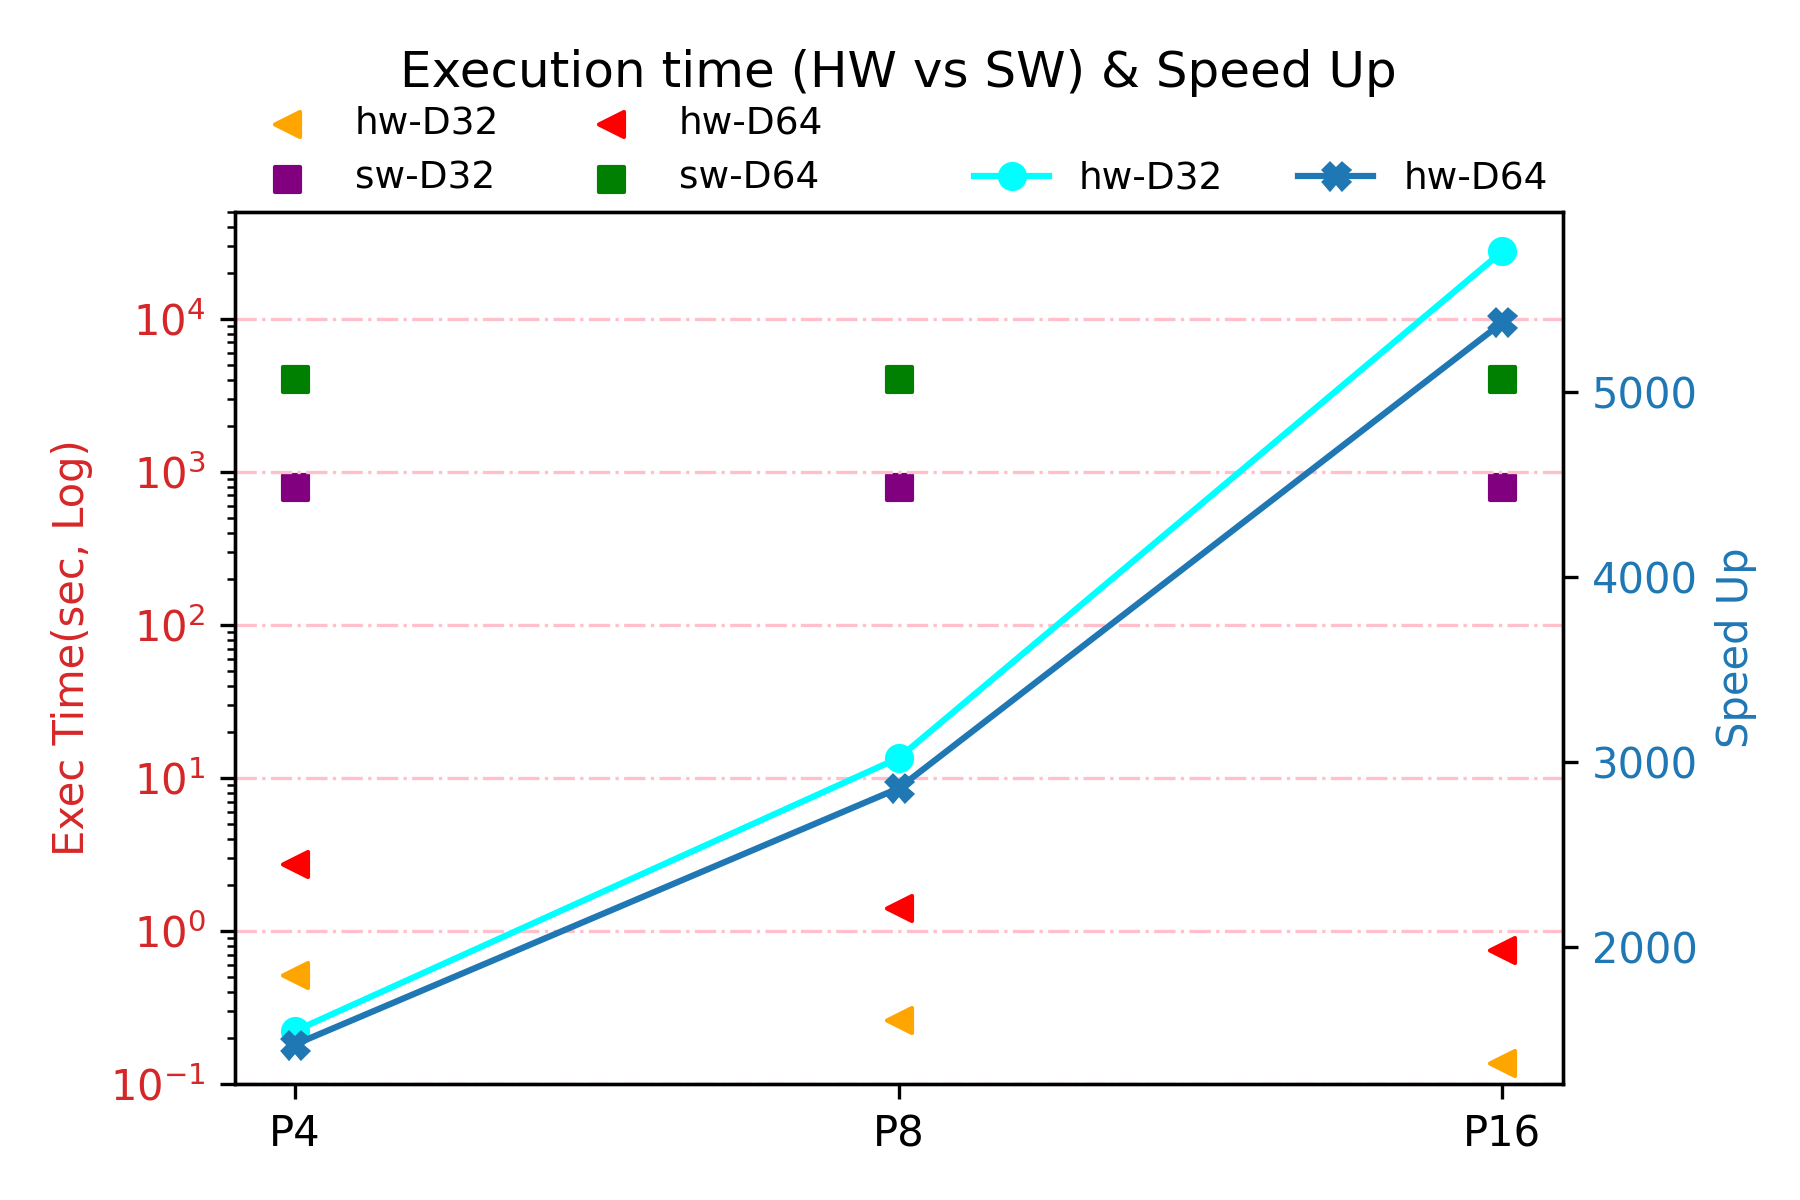
\includegraphics[width=\columnwidth]{figure/a0-both.png}
    \caption{Latency comparison of D32 and D64 Dataset}
    \label{fig-d32-64}
\end{figure}

For A1 architecture, latency results are shown in Fig.\ref{fig-a1-x} and Fig.\ref{fig-a1-k}. For 128x128x128 dataset, numX = numK = 2048K. To evaluation the speedup of accelerator with A1 architecture, I tested P4\_A1\_DMA64. As we discussed in section 3.3, parallel level in compute process won't affect latency performance, so we choose the P4 accelerator. (It is possible that there is a parallelism level which is smaller than 4 and can also balance the loading and computing processes to further reduce area while with the same latency performance.).The speed-up value is increasing when increasing the data size. Fig.\ref{fig-a1-x} shows the execution time comparison of software and hardware and speedup when numK is fixed at 4K and numX is increasing. Fig.\ref{fig-a1-k} shows how execution time and speedup change over numK increasing from 4K to 256K while numX is fixed as 4.  At some point, speedup saturates when numK and numX increases. For our A1 architecture, we get at least 400 times acceleration compared with software execution for any arbitrary input image size.\\

\begin{figure}[h!]
    \centering
    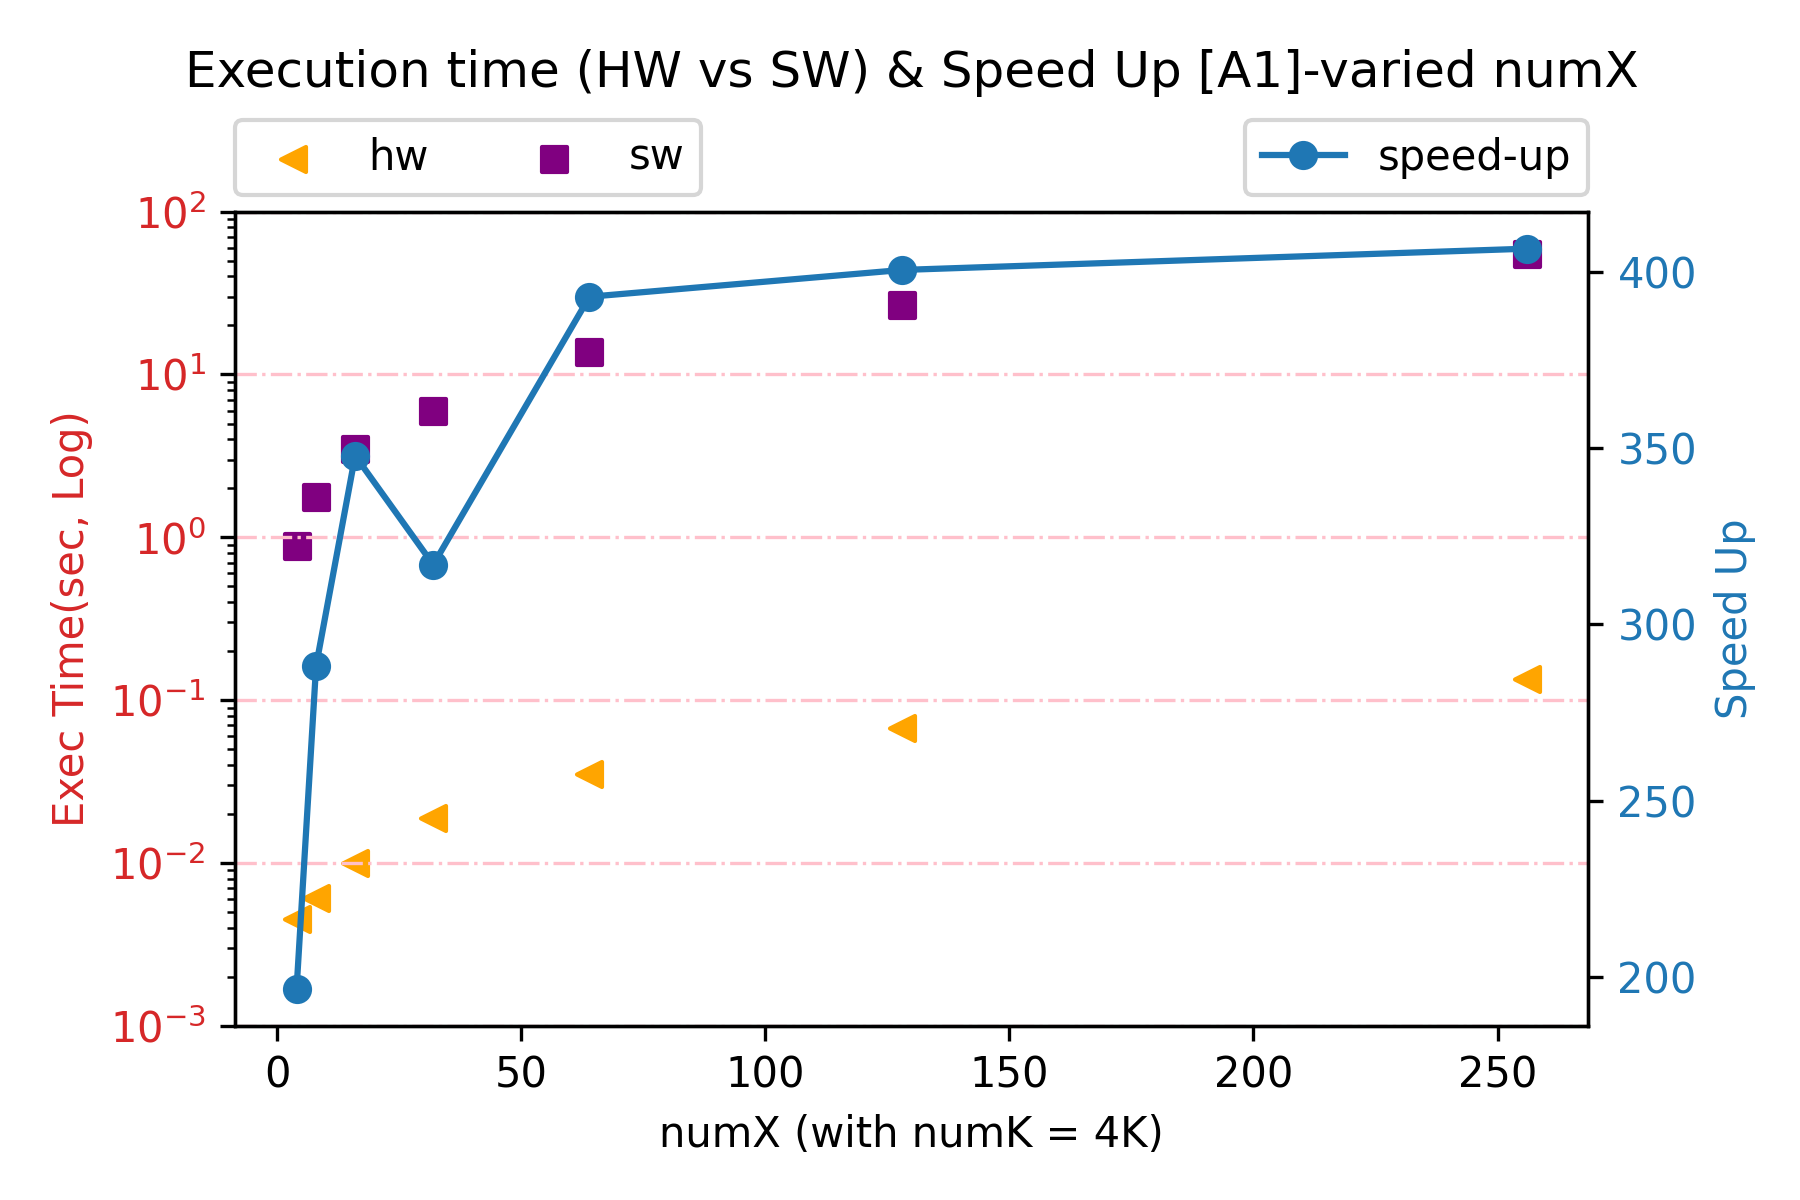
\includegraphics[width=\columnwidth]{figure/a1-vary-x.png}
    \caption{Latency with varying numX (numK=4K)}
    \label{fig-a1-x}
\end{figure}

\begin{figure}[h!]
    \centering
    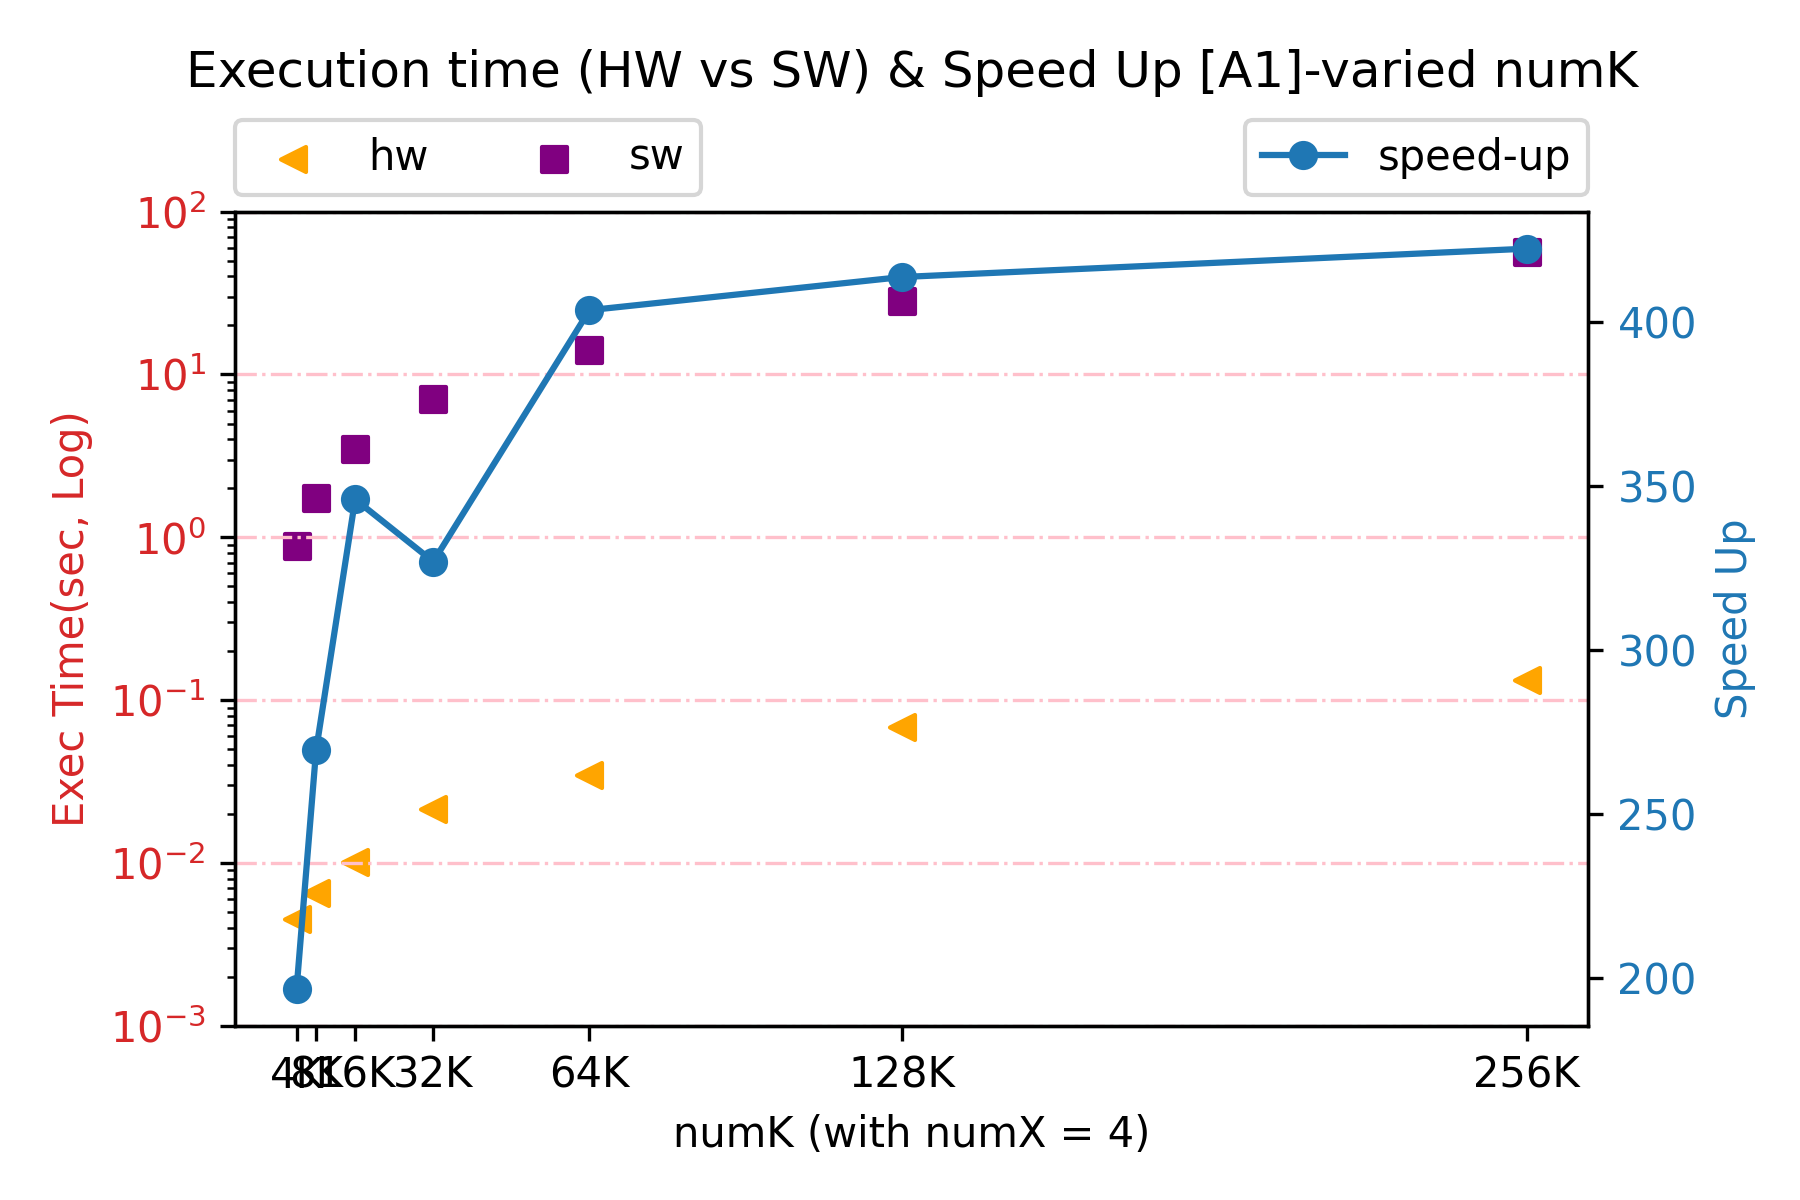
\includegraphics[width=\columnwidth]{figure/a1-vary-k.png}
    \caption{Latency with varying numK (numX=4)}
    \label{fig-a1-k}
\end{figure}



\section{Conclusion}
In this project, I have designed a set of accelerators using ESP to compute the Q matrix for MRI image reconstruction. Any arbitrary input data sizes can find an accelerator to work with. The accelerators are tested on the FPGA through both bare-metal application and Linux application. I have also done different levels of design space exploration. Customizing PLM designs and reducing the fixed point precision can reduce both area and latency. Loop-unrolling and loop-pipelining in the main computation-intensive loop can reduce latency proportionally when compute kernel is dominating the whole procedure. 

\section{Limitations of The Work}

We don't compare our acceleration result with the state-of-the-art MRI image recustruction performance since we only accelerate one part of the iamge reconstruction. The whole image recustruction of non-Cartician scanning contains three steps: computing Q-matrix, computing the vector $\mathbf{F}^{H} \mathbf{d}$, and finding the image iteratively via a conjugate gradient linear solver. The first two steps are very similiar.~\cite{stone2008accelerating} Since our accelerator only accelerate the first step, we can't evaluate the reconstructed image quality and the performance with other works. Also, we don't know the error tolerance of the first step. 


\section{Potential Future Work}
\begin{itemize}
    \item Design the same set of accelerators with Vivado HLS C/C++ through ESP for the MRI-Q matrix computation. Compare the latency and area performance between the generated RTLs through two different design flows.
    \item Design accelerators to compute the second step mentioned in Section 6. 
\end{itemize}



%Bibliography
{\small
\balance
%\bibliographystyle{abbrv}
\bibliographystyle{unsrt}
\bibliography{ref}
}


% If you need to add an appendix with large figures or table use the following
% code:

%% \newpage
%% \onecolumn{
%% \centering
%% \section*{APPENDIX}
%% \vspace{0.5in}

%% % Add your Appendix text and figures here.

%% }

\end{document}
